\documentclass[11pt]{article}
\usepackage[margin=1.0in]{geometry}
\addtolength{\topmargin}{0.25in}
\usepackage[document]{ragged2e}
\usepackage{graphicx}
\graphicspath{{../pictures/}}
\usepackage{float}
\usepackage{siunitx}

\begin{document}
	{\Huge\textbf{EEE381 Tech Memo}}\\
	\hfill \break
	\textbf{From:} Charles Noah Lutz\\
	\textbf{Partner:} N/A\\
	\textbf{To:} Colin Bussert\\
	\textbf{Date:} Performed: 11/29/18; Due: 12/09/18\\
	\textbf{Subject:} Lab \#05-06

	\section{Abstract}
	The goal of lab exercises 5 and 6 was to build a functioning operational amplifier
	and observe several different characteristics of the op-amp. These characteristics
	included gain of each individual stage, the overall gain and the frequency response
	of the overall op-amp. The circuit was first designed using hand calculations, then
	tested in a PSPICE simulator to verify the operation. Then the op-amp was built in-lab
	and tested experimentally. 
	
	\section{Theory}
	An ideal op-amp has an input resistance of infinity, an output resistance
	of zero and a gain of infinity. While this is not practically possible, the closer an op-amp can be 
	built to the ideal case, the better the op-amp will perform in any given circuit.
	The two amplifiers that were used in this lab exercise was the NMOS differential amplifier 
	(effectivly two common source amplifiers) with a PMOS current mirror load and a PMOS
	common source amplifier. Figure \ref{fig:op-amp} shows the schematic for the op-amp. \\
	\begin{figure}[H]
		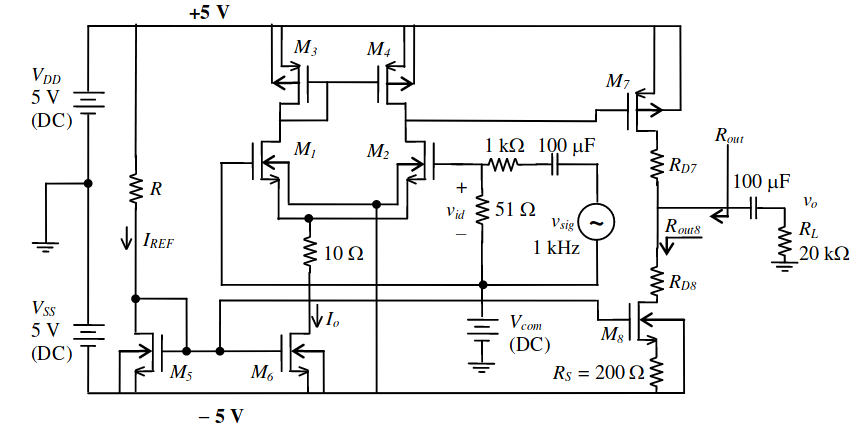
\includegraphics[width=\textwidth]{op_amp_schematic.png}
		\caption{Operational amplifier used for this lab exercise}
		\label{fig:op-amp}
	\end{figure}
	
	The first value that was calculated was the reference current that was required
	to ensure that the op-amp had a gain of $>$ 240 $\frac{\si\volt}{\si\volt}$. Using the
	differential amplifier that was built in lab exercise 4 as a starting point, which had a
	reference current of 4$\si{\milli\ampere}$, the only thing that needed to be calculated
	was the effective gain when the two stages are cascaded. 

	\begin{equation}
		A_{v} = A_{1} * A_{2} = -33.665 * -25.668 = 864.1132 \frac{\si{\volt}}{\si{\volt}}
	\end{equation}

	As the calculated gain is much more than 240$\frac{\si\volt}{\si\volt}$ it was decided
	to go with 4$\si{\milli\ampere}$ as the reference current. \\
	\hfill\break

	The next values that needed to be calculated were the $R_{7/8}$ values to center 
	the output around 0$\si\volt$ DC. It was found that to center the output $R_8$ to
	2.15$\si{\kilo\ohm}$. Since this value needed to be a standard resistor value, a
	resistor of 2.2$\si{\kilo\ohm}$ was used. \\
	\hfill\break

	Next, the circuit was built and simulated in PSPICE. Figure \ref{fig:pspice_opamp}
	shows the circuit in PSPICE.

	\begin{figure}[H]
		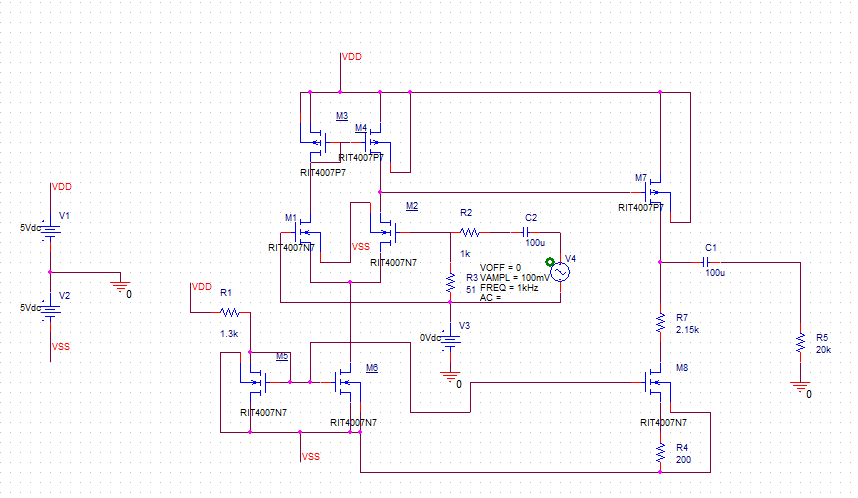
\includegraphics[width=\textwidth]{op_amp.png}
		\caption{Operational amplifier in PSPICE simulator}
		\label{fig:pspice_opamp}
	\end{figure}

	The first simulation that was run was a simple transient simulation to find the 
	overall gain of the amplifier. Figure \ref{fig:pspice_gain} shows the input
	signal and the output signal. 

	\begin{figure}[H]
		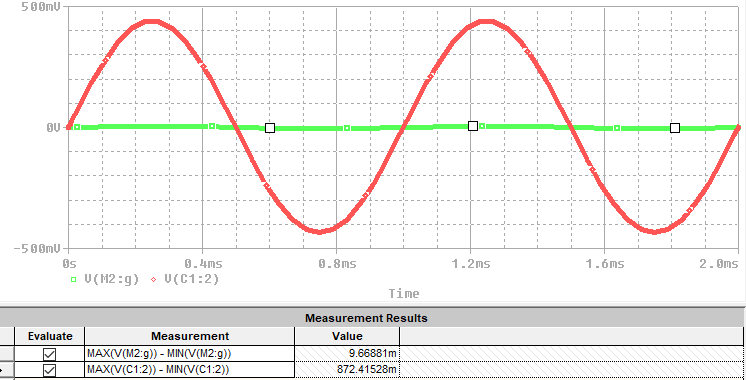
\includegraphics[width=\textwidth]{voltage_gain.png}
		\caption{PSPICE simulated voltage gain of operational amplifier}
		\label{fig:pspice_gain}
	\end{figure}

	\begin{equation}
		A_v = \frac{V_{out}}{V_{in}} = \frac{872.415\si{\milli\volt}}{9.669\si{\milli\volt}} = 90.228 \frac{\si\volt}{\si\volt}
	\end{equation}

	The next simulation that was run was a frequency response. The frequency of the input was varied
	from 1$\si\hertz$ to 100$\si{\mega\hertz}$ and gain measured and graphed against the frequency. 
	Figure \ref{fig:freq_response} shows the gain (in dB) versus the frequency of the input signal.

	\begin{figure}[H]
		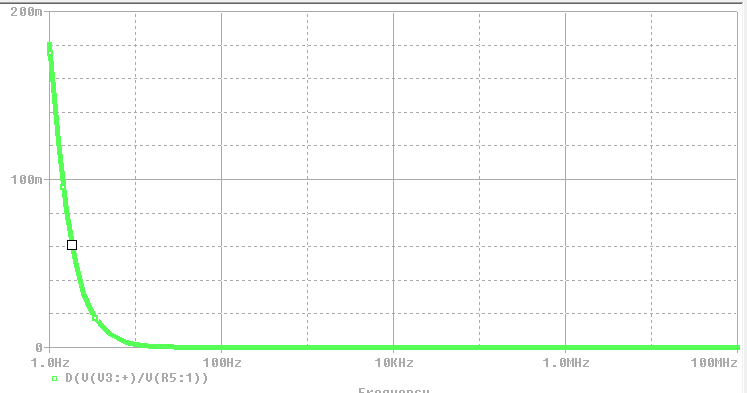
\includegraphics[width=\textwidth]{frequency_response.png}
		\caption{Simulated frequency response of op-amp}
		\label{fig:freq_response}
	\end{figure}
	
	It should be noted that this frequency response graph is incorrect and could 
	be due to the simulation profile being set up incorrectly or the transistor values
	being incorrect. 

	\section{Results and Discussion}
	Next, the circuit in Figure \ref{fig:op-amp} was built in-lab using CD4007
	packages and a breadboard. The differential pair that was built in lab excercise 4
	was used as a starting point and modified slightly to add the second common source
	amplifier.\\
	\hfill\break

	First the overall gain of the circuit was measured. This was done using a waveform generator
	running at 1$\si{\kilo\hertz}$ and an oscilloscope to measure the output.
	Figure \ref{fig:experimental_gain} shows the experimental gain where channel 1 shows input and 
	channel 2 shows output.

	\begin{figure}[H]
		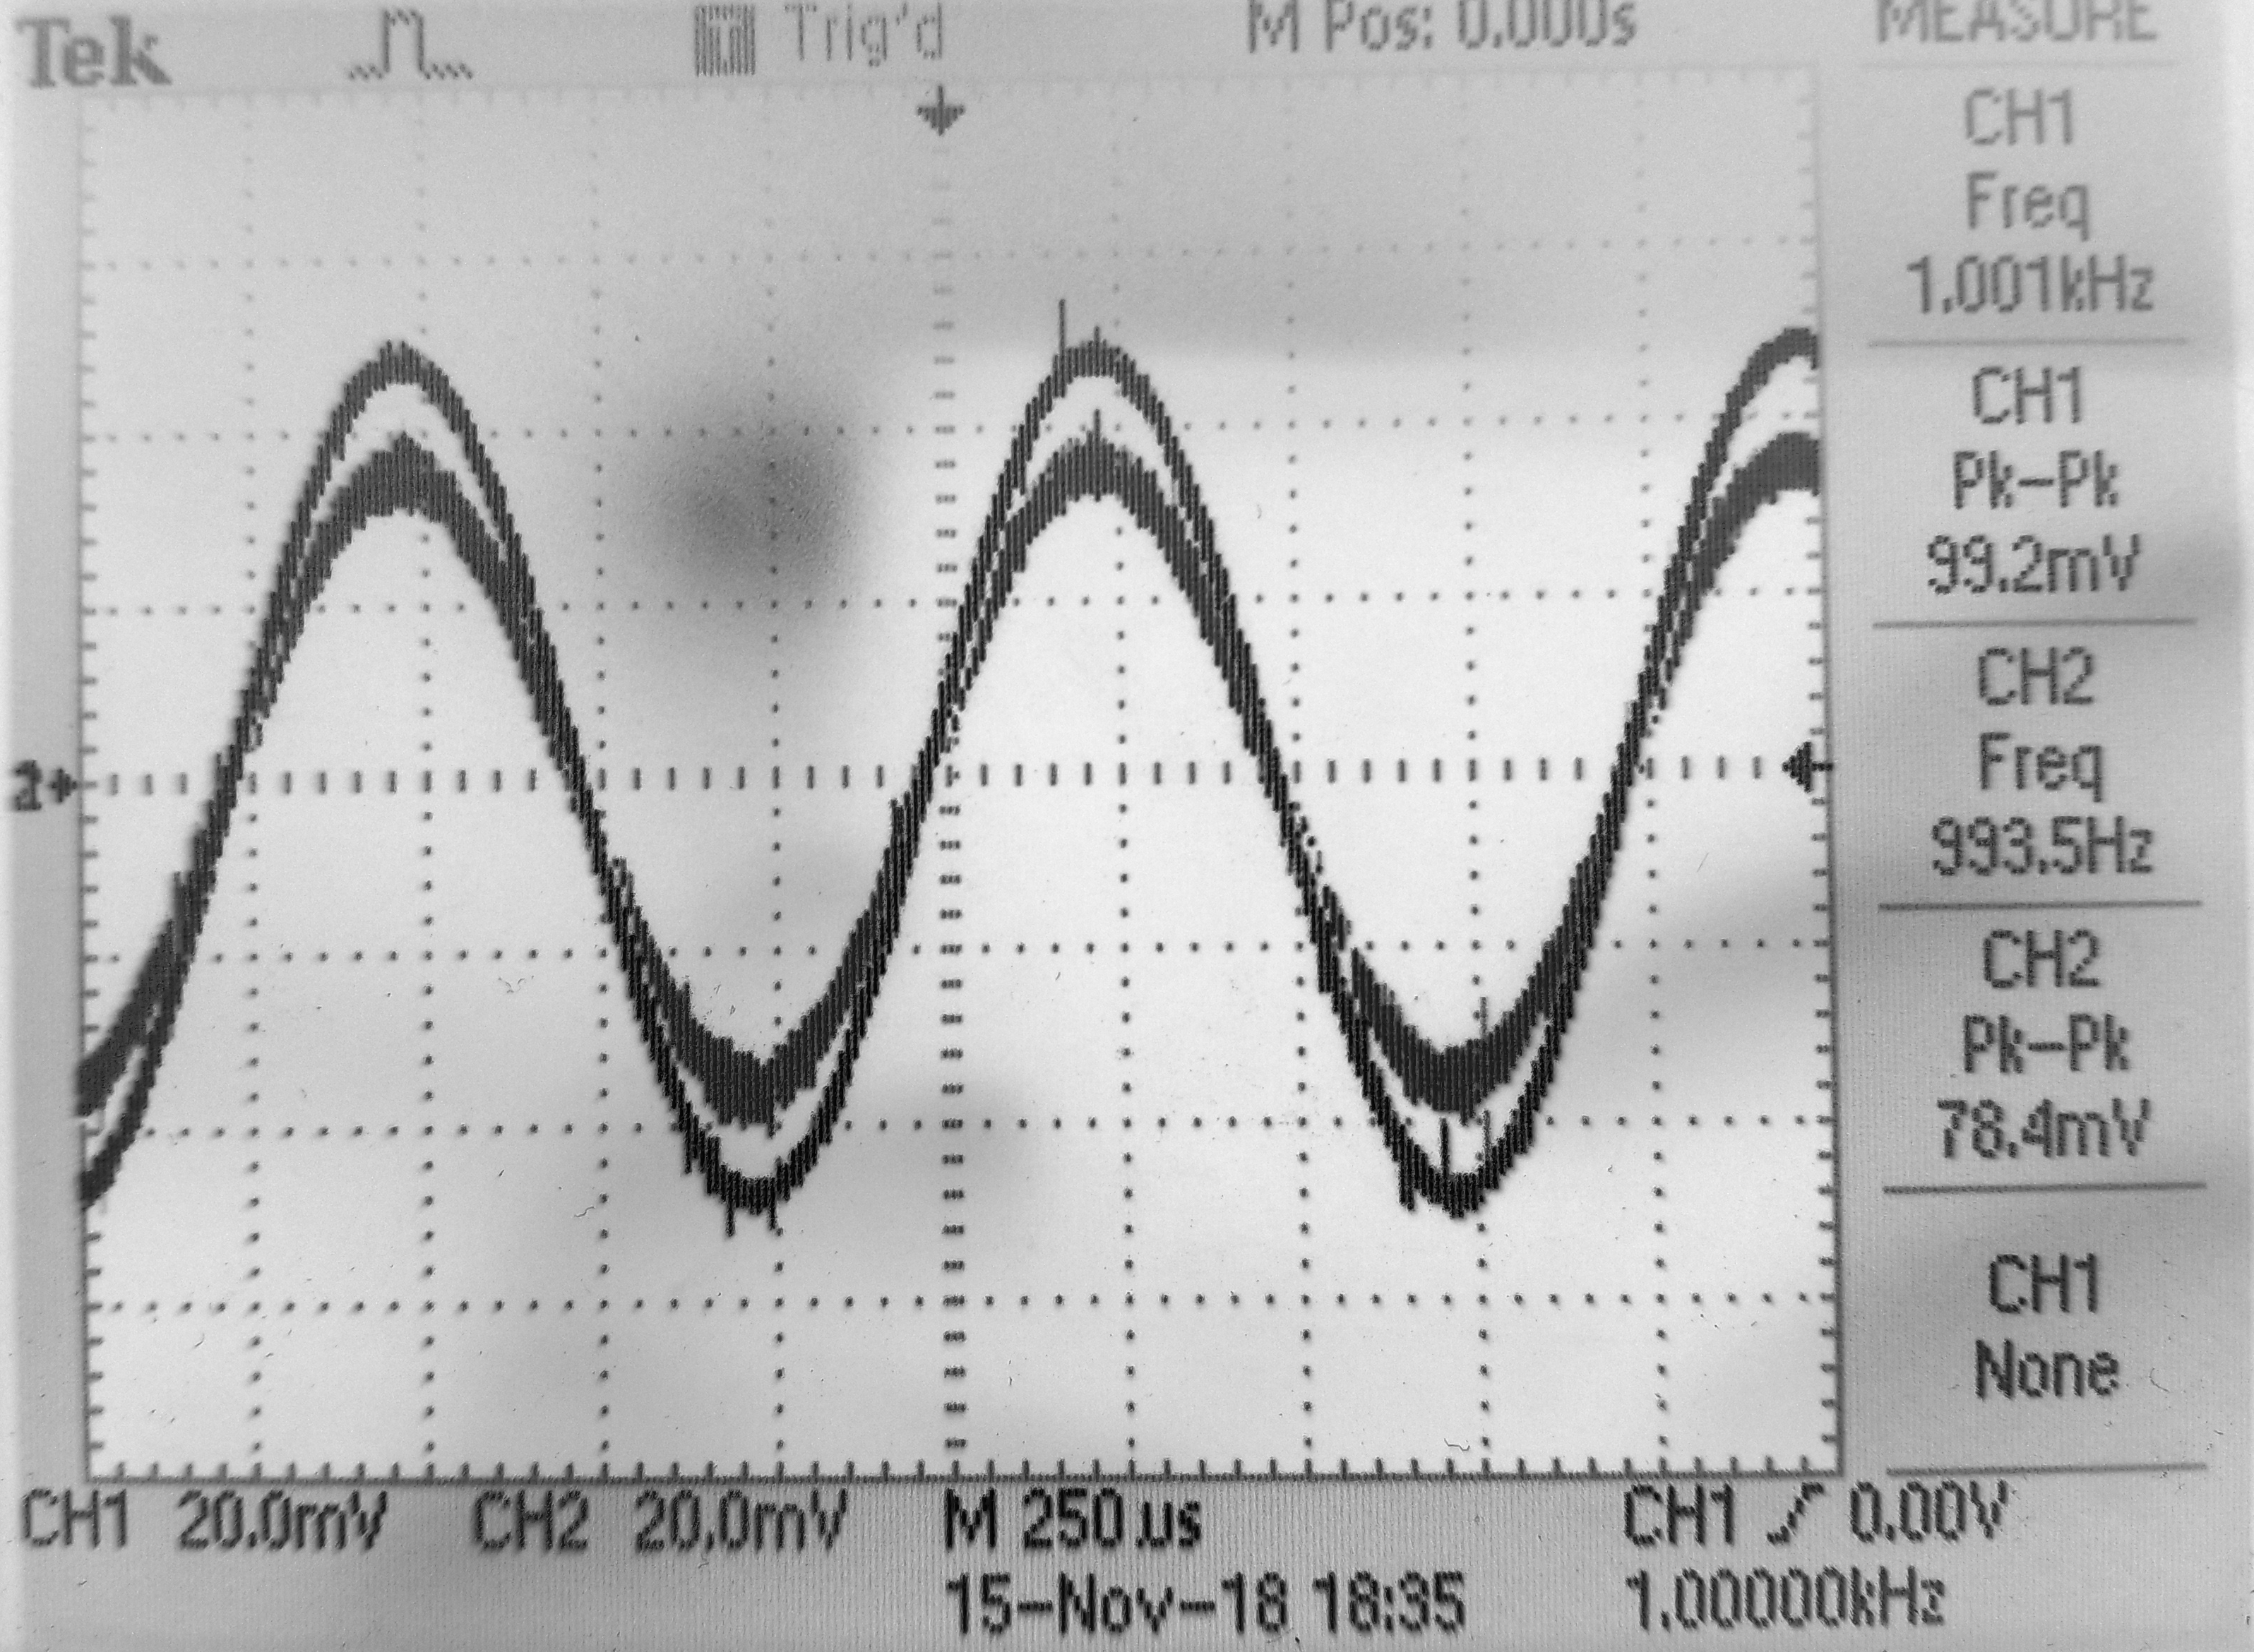
\includegraphics[width=\textwidth]{experimental_gain.jpg}
		\caption{Experimental gain}
		\label{fig:experimental_gain}
	\end{figure}

	It should be noted that we could not get our second stage (common source amplifier)
	working. Instead we used the first stage as our output. This results in a much lower
	gain, as it is only going through one amplifier. \\
	\hfill\break
	
	\begin{table}[H]
		\centering
		\caption{Experimental gain measurements}
		\label{table:exp_gain}
		\begin{tabular}{|c|c|}
			\hline
			\textbf{Voltage} & \textbf{Value}\\
			\hline
			$V_{sig}$ & 99.2 $\si{\milli\volt}$\\
			$V_{id}$ & 4.813 $\si{\milli\volt}$\\
			$V_o$ & 78.4 $\si{\milli\volt}$\\
			\hline
		\end{tabular}
	\end{table}
	\begin{equation}
		A_v = \frac{V_{out}}{V_{id}} = \frac{78.4\si{\milli\volt}}{4.813\si{\milli\volt}} = 16.29 \frac{\si\volt}{\si\volt}
	\end{equation}

	Next, the frequency response of the circuit was tested. Again, a waveform generator 
	running at various frequencies was used for input and an oscilloscope was used to measure the 
	input and output which was used to calculate the gain in dB. Table \ref{table:exp_freq_response}
	shows the raw data and Figure \ref{fig:exp_freq_response} shows the logarithmic graph for 
	frequency response.

	\begin{table}[H]
		\centering
		\caption{Experimental frequency response data}
		\label{table:exp_freq_response}
		\begin{tabular}{|c|c|}
			\hline
			\textbf{Frequency} & \textbf{Gain (dB)}\\
			\hline
			100 $\si\hertz$ & 25.105\\
			1 $\si{\kilo\hertz}$ & 25.105\\
			10 $\si{\kilo\hertz}$ & 25.015\\
			100 $\si{\kilo\hertz}$ & 20\\
			1 $\si{\mega\hertz}$ & 7.61\\
			10 $\si{\mega\hertz}$ & 2.11\\
			\hline
		\end{tabular}
	\end{table}

	\begin{figure}[H]
		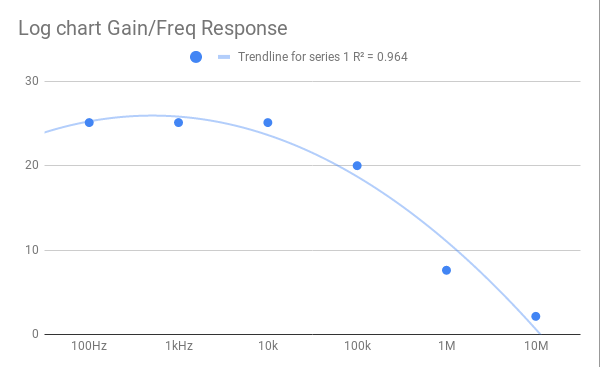
\includegraphics[width=\textwidth]{experimental_freq_response.png}
		\caption{Experimental frequency response Bode plot}
		\label{fig:exp_freq_response}
	\end{figure}

	As the frequency gets above 10 $\si{\kilo\hertz}$, the gain starts to drop off.
	This is not consistent with the frequency response graph that was obtained during
	PSPICE simulation. This could be due to the simulation profile being set up incorrectly, 
	returning incorrect values. This theory is supported by the fact that the simulated
	frequency response graph was not the correct general shape. 

	\section{Conclusion}
	The goal of lab exercise 5 and 6 was to build a functioning operational amplifier
	using a differential amplifier and a common source amplifier. The specific attributes
	of the amplifier that were being investigated were the overall gain of the amplifier
	and the frequency response. \\

	During the in-lab portion of the exercise we were unable to get the second stage,
	common source amplifier to sucessfully work, due to this, we instead used the first stage, 
	differential amplifier as our output. While this reduced our overall gain, it still allowed
	us to run a frequency analysis on the amplifier. \\

	There was also an error during simulation that caused the simulated frequency response
	to be incorrect. This could have been due to the transistors being set up wrong or the 
	simulation profile being incorrect. 

\end{document}
